\documentclass{article}
\usepackage{stmaryrd}
\usepackage{graphicx}
\usepackage{float}
\title{Report, Kinetic project}
\author{Dorian Geraldes Pereira, Axel Demuth}
\date{March 2024}

\begin{document}
\maketitle
\tableofcontents
\newpage
\section{Project Objective}

Within this project scope, the primary goal is to implement an efficient and accurate 
conversion process for Industry Foundation Classes (IFC) 
files representing buildings or cities into meshes compatible with the 
Kinetic algorithm. Subsequently, the Kinetic algorithm will be applied to these 
meshes to produce watertight models, facilitating the execution of finite element calculations.

The specific steps to be undertaken are as follows:

\begin{enumerate}   
    \item \textbf{Mesh Conversion:} From the IFC files we will have a 
    conversion in the stl or msh format,we will need to convert the STL 
    or MSH meshes into one of the formats accepted by the Kinetic algorithm, 
    such as .ply, .xyz, .las, .off.
    
    \item \textbf{Application of the Kinetic Algorithm:} Applicate  
    the Kinetic algorithm on the the converted 
    meshes to produce meshes optimized for finite element calculations.
    
    \item \textbf{Recovery of Material Labels:} Ensure the preservation 
    of information regarding materials present in the initial IFC-format mesh 
    and correctly associate them with elements of the converted mesh.
    
    \item \textbf{Utilization on City Modeling:} Extend the application of 
    the Kinetic algorithm to entire city models.
\end{enumerate}

\section{Current Project Challenges}

Currently, the project faces several technical challenges:

\begin{enumerate}
    \item \textbf{Mesh Conversion:} Find a solutions to convert meshes 
    from STL or MSH files into one of the formats accepted by the Kinetic algorithm.
    
    \item \textbf{Parameter Optimization:} Identify and adjust appropriate 
    parameters to avoid segmentation faults and achieve satisfactory results 
    when applying the Kinetic algorithm.
    
    \item \textbf{Version Differences:} Understand the distinctions between 
    versions of the Kinetic algorithm,developed by CGAL and INRIA, to select 
    the right parameters to get the best result
\end{enumerate}

By overcoming these challenges, the project aims to provide a 
comprehensive and efficient solution for analyzing urban structures 
using the Kinetic algorithm to facilitate finite element calculations.\newline

\section{Tools}
\subsection{CGAL}
CGAL is a comprehensive package for geometry algorithms, providing various data structures and algorithms for working on polygons, surfaces, mesh generation, and more.
It offers a wide range of functionalities for geometric processing and analysis in various fields such as computer graphics, computational geometry, and geometric modeling.
\subsection{Kinetic}

Kinetic algorithms is a package from CGAL that allows working on meshes with some holes in them. When applied to the mesh, the Kinetic algorithms will 'extend' some surfaces to fill the mesh and make it watertight. 
Here's what the algorithm is capable of:


\begin{figure}[h]
    
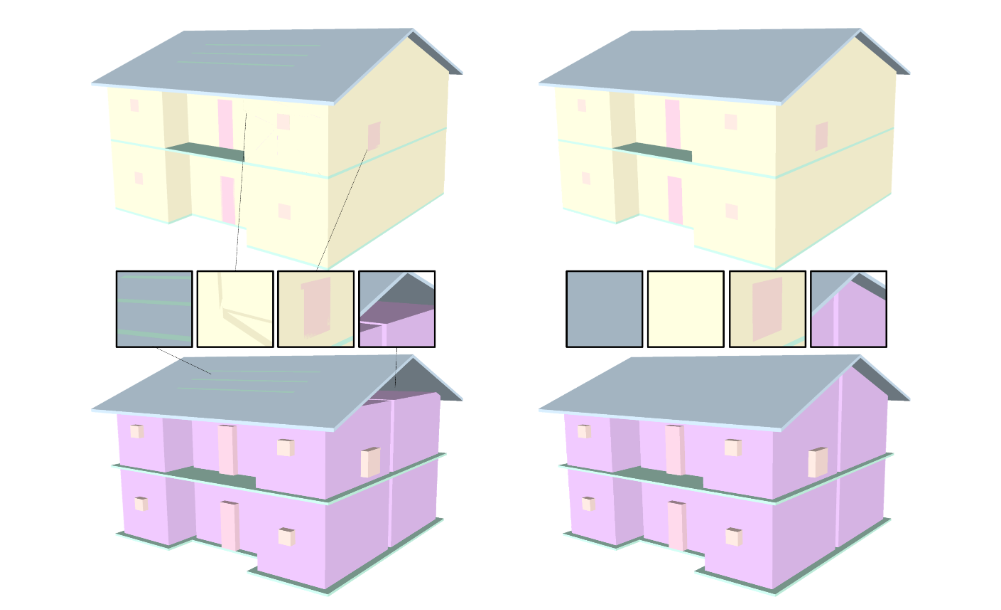
\includegraphics[scale =   0.3 ]{../../images/example_algorithm.png}

\end{figure}


To utilize the algorithm, we employ one from CGAL. Given a set of parameters and a file containing a point cloud along with the associated normals to the points,
the algorithm is applied. We were fortunate to have a meeting with Florent Lafarge, one of the creators of the algorithm,
who explained to us which parameters are crucial for analysis and how each one can significantly influence the results.
Two parameters stand out as particularly important: 
\begin{itemize}
  \item 'dist' indicates the distance between two points required to consider them for plane construction.
  \item 'pmin' represents the number of points used to construct a plane.
\end{itemize}

In order to understand how these parameters affect the outcome, we will examine the same point cloud while varying the value of 'pmin' first and then varying 'dist.'
The algorithm produces .off files as output, which can be visualized using software such as MeshLab.

\newpage
The original point cloud represents this building:
\vspace{\baselineskip}

\begin{center}
    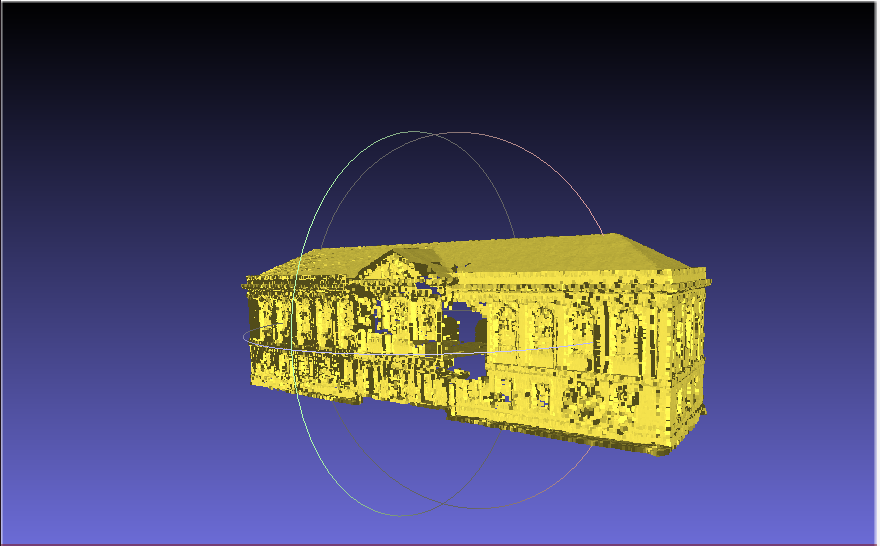
\includegraphics[scale=0.20]{../../images/screen_kinetic/building.png} 
\end{center}



\begin{figure}[H]
    \centering
    \begin{minipage}[b]{0.45\textwidth}
      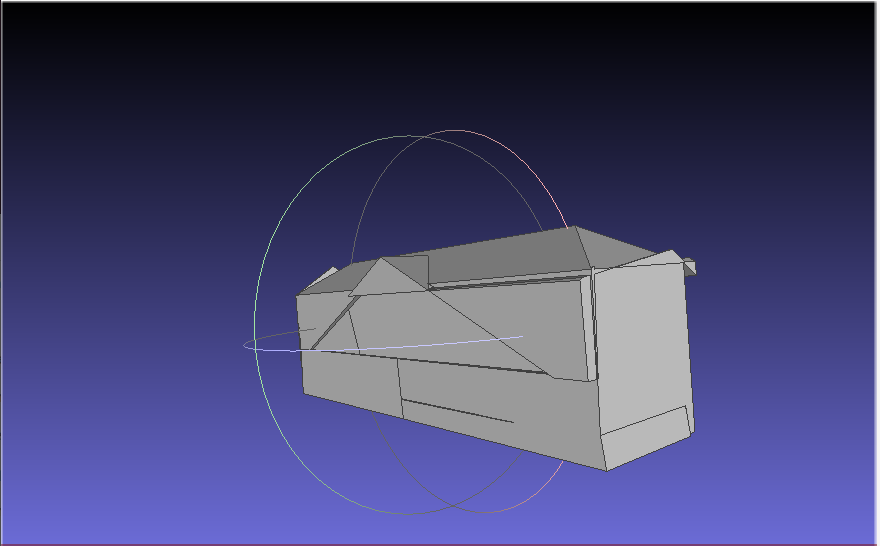
\includegraphics[width=\textwidth]{../../images/screen_kinetic/dist1_pmin220.png}
      \caption{dist1\_pmin220}
      \label{fig:dist1_pmin220}
    \end{minipage}
    \hfill
    \begin{minipage}[b]{0.45\textwidth}
      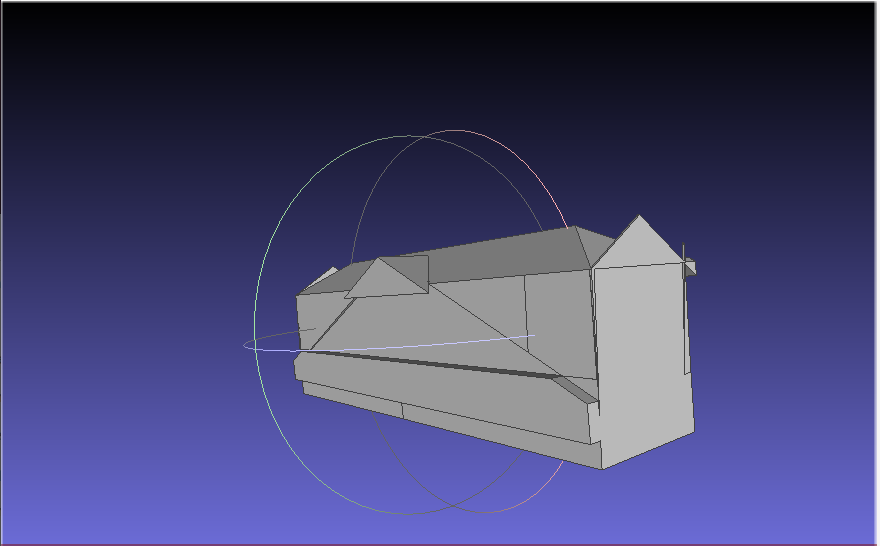
\includegraphics[width=\textwidth]{../../images/screen_kinetic/dist1_pmin250.png}
      \caption{dist1\_pmin250}
      \label{fig:dist1_pmin250}
    \end{minipage}
    \hfill
    \begin{minipage}[b]{0.45\textwidth}
      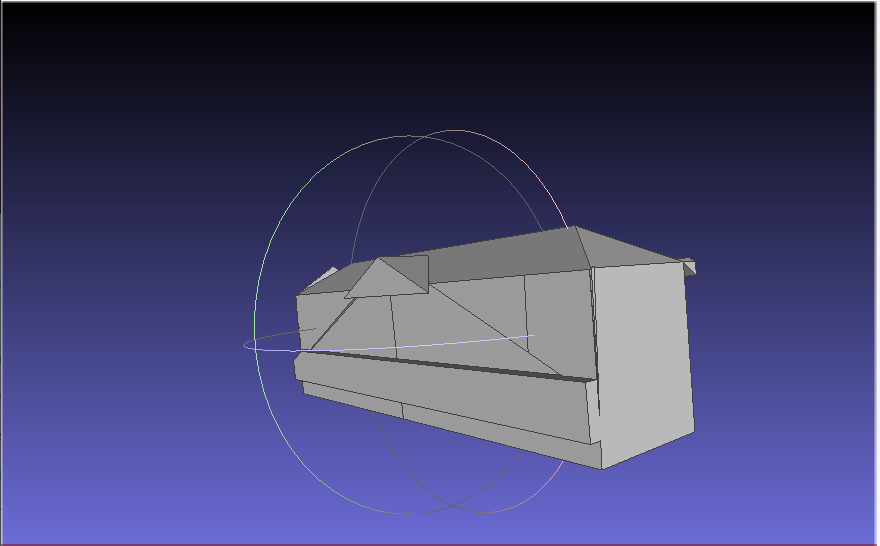
\includegraphics[width=\textwidth]{../../images/screen_kinetic/dist1_pmin280.png}
      \caption{dist1\_pmin280}
      \label{fig:dist1_pmin280}
    \end{minipage}
    \hfill
    \begin{minipage}[b]{0.45\textwidth}

        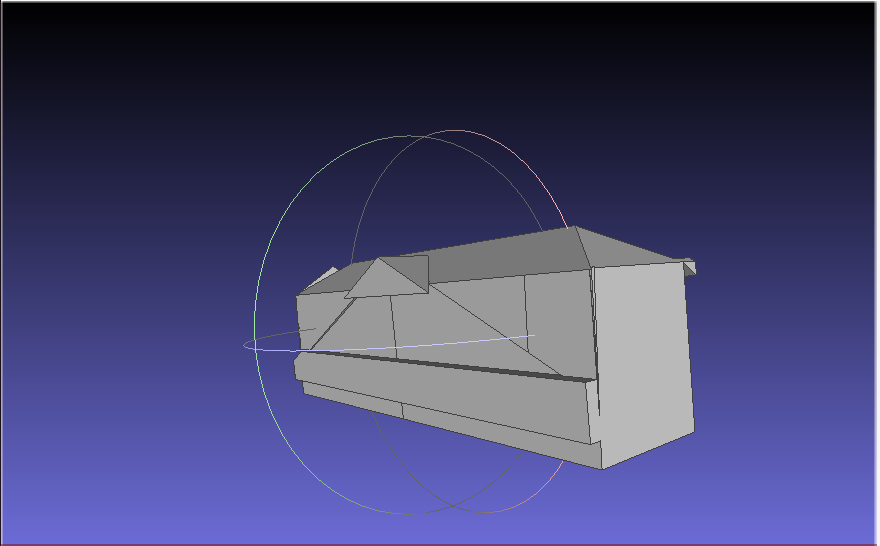
\includegraphics[width=\textwidth]{../../images/screen_kinetic/dist1_pmin300.png}
        \caption{dist1\_pmin300}
        \label{fig:dist1_pmin300}
      \end{minipage}
  \end{figure}
  
  First, it's important to understand that setting 'pmin' too low can lead to errors. Subsequently,if 'pmin' is too small, we may not capture enough structural detail,
  whereas setting 'pmin' too high may cause planes to overlap, resulting in loss of information



  \begin{figure}[H]
    \centering
    \begin{minipage}[b]{0.45\textwidth}
      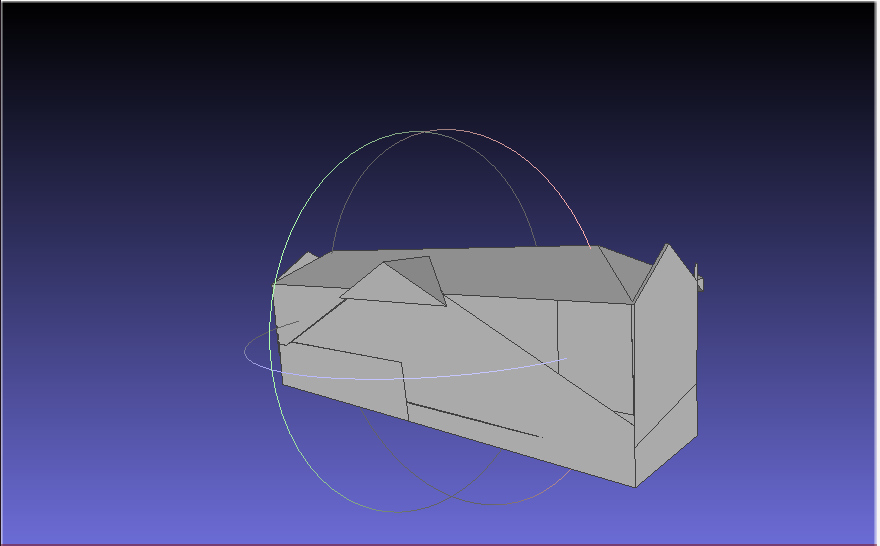
\includegraphics[width=\textwidth]{../../images/screen_kinetic/dist1_5_pmin_250.png}
      \caption{dist15\_pmin250.png}
      \label{fig:dist15_pmin220}
    \end{minipage}
    \hfill
    \begin{minipage}[b]{0.45\textwidth}
      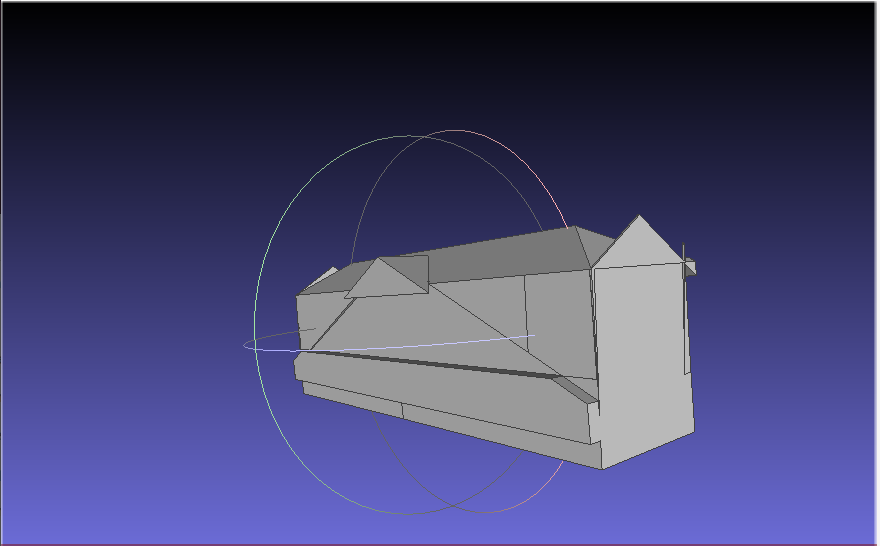
\includegraphics[width=\textwidth]{../../images/screen_kinetic/dist1_pmin250.png}
      \caption{dist1\_pmin250}
      \label{fig:dist1_pmin250}
    \end{minipage}
    \hfill
    \begin{minipage}[b]{0.45\textwidth}
      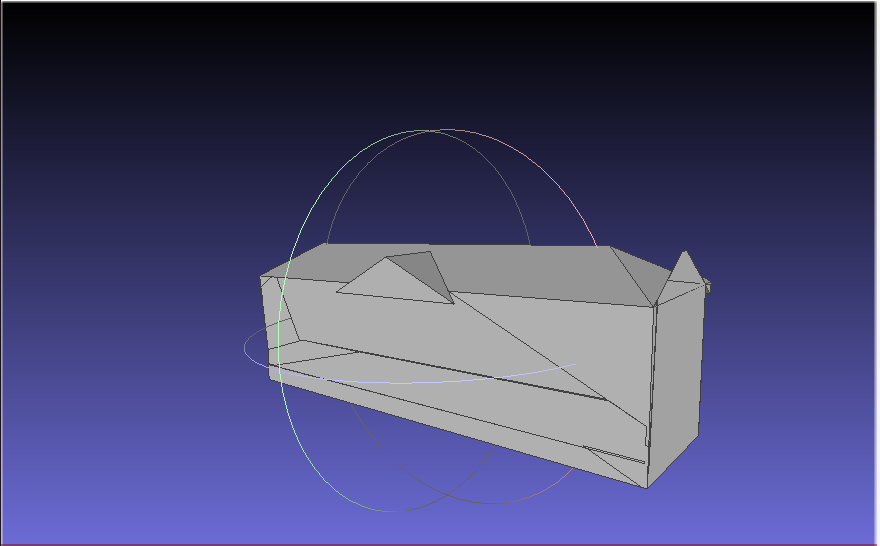
\includegraphics[width=\textwidth]{../../images/screen_kinetic/dist_0_3_pmin_250.png}
      \caption{dist03\_pmin250}
      \label{fig:dist03_pmin250}
    \end{minipage}
    \hfill
    \begin{minipage}[b]{0.45\textwidth}

        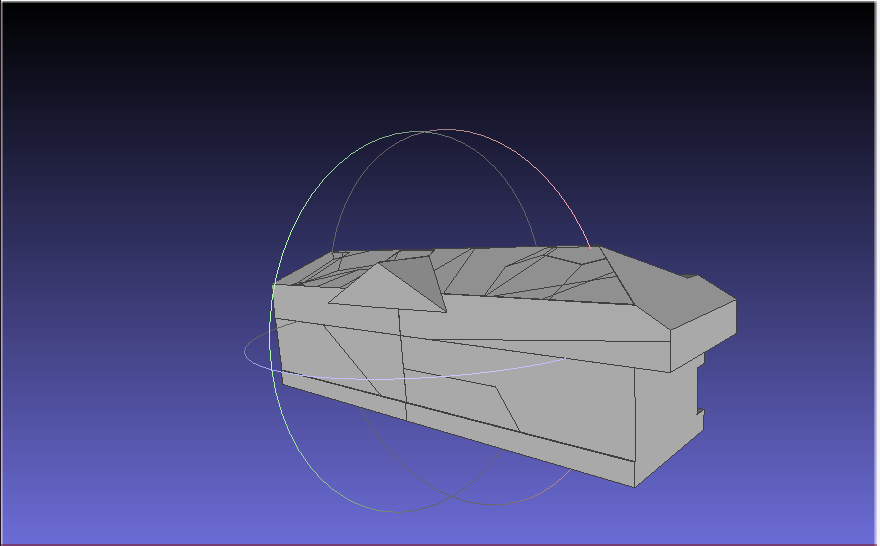
\includegraphics[width=\textwidth]{../../images/screen_kinetic/dist_001_pmin_250.png}
        \caption{dist001\_pmin250}
        \label{fig:dist1_pmin300}
      \end{minipage}
    \begin{minipage}[b]{0.45\textwidth}

        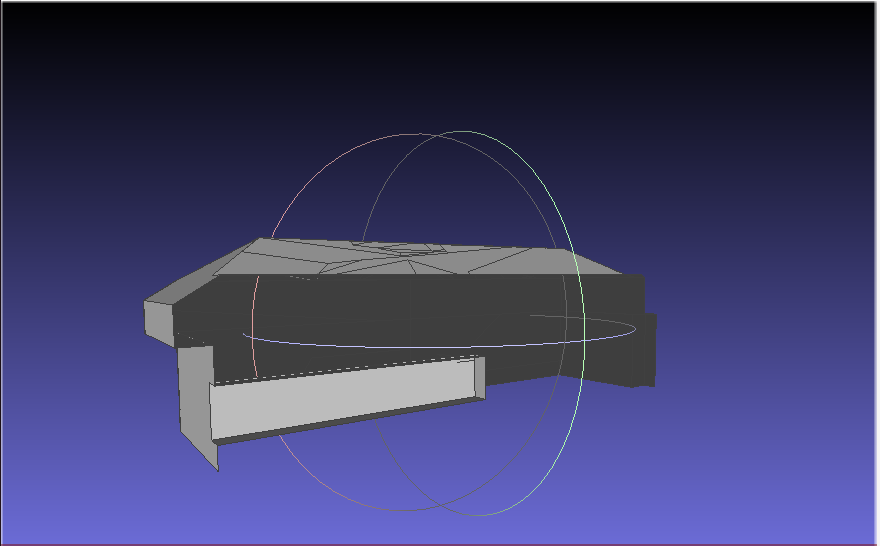
\includegraphics[width=\textwidth]{../../images/screen_kinetic/back_dist001_pmin250.png}
        \caption{dist001\_pmin250}
        \label{fig:dist1_pmin300}
      \end{minipage}
  \end{figure}


  When considering the 'dist' parameter, if it is set too high, we risk losing significant structural details. 
  In the opposite, if the distance is too small, surfaces may be divided into too many planes, potentially resulting in an incomplete coverage of the entire mesh, 
  as observed at the rear of the building with a 'dist' of 0.001.

  One of the challenges in studying this algorithm is determining the appropriate 'qmin' and 'dist' to achieve the desired number of space partitions.
  Setting it too high may enhance precision but extend execution time, and in some cases, incorrect values can lead to program crashes.

This algorithm could be a crucial tool in our project, particularly when dealing with massive meshes for large buildings,
hospitals, etc. When creating large meshes, issues can arise, and errors within the mesh can be detrimental during simulations,potentially leading to false results. 
This algorithm allows us to rectify such mesh problems.

One limitation of the algorithm is its input requirement, as it currently only works with scatter plots. Consequently, we are unable to utilize the IFC format, 
resulting in the loss of valuable information regarding the types of structures present. To address this limitation, 
we plan to implement a process involving the conversion of IFC to scatter plot with associated data, followed by conversion to formats such as .plt, .ply, .xyz,
which are supported by Kinetic CGAL, ultimately resulting in a mesh with associated data.


\section{Analysis of Results}

Analysis of the final meshes reveals significant differences between those produced by the CGAL algorithm and those generated by the INRIA algorithm. The final mesh obtained with CGAL demonstrates satisfactory watertightness but is characterized by noticeable roughness. Conversely, the final mesh generated by the INRIA algorithm is remarkably smoother, offering a more uniform surface.

\subsection{Visualization of Results}

For better visual understanding, three images are provided below:

\begin{itemize}
    \item Initial point cloud
    \item Result of the mesh with the CGAL algorithm
    \item Result of the mesh with the INRIA algorithm
\end{itemize}

\vspace{0.5cm}
\begin{figure}[h]
\centering
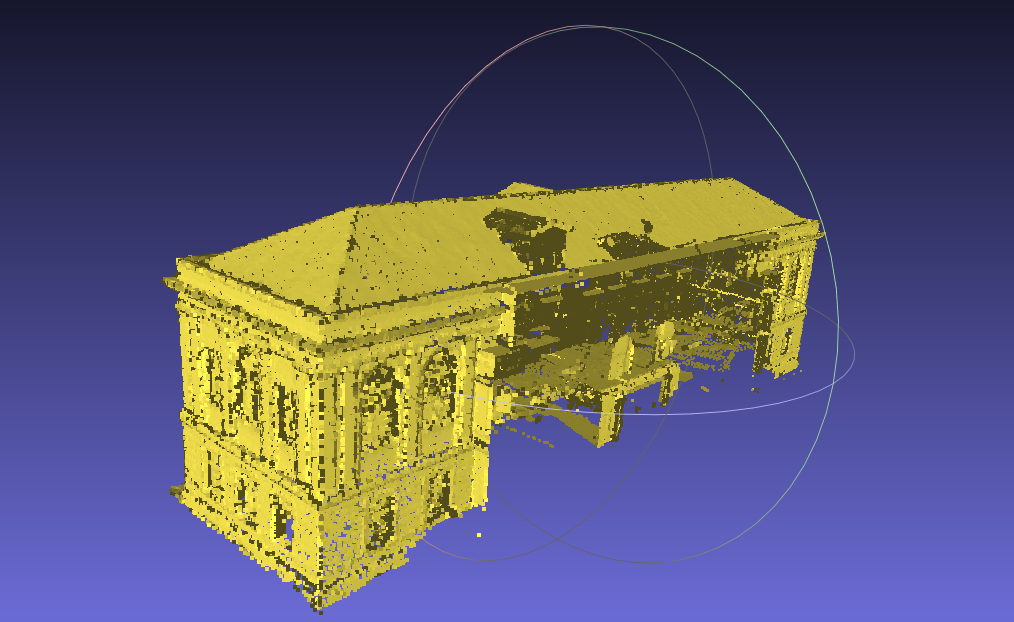
\includegraphics[width=0.25\textwidth]{../../images/screen_kinetic/building_point.png}
\hspace{0.05\textwidth}
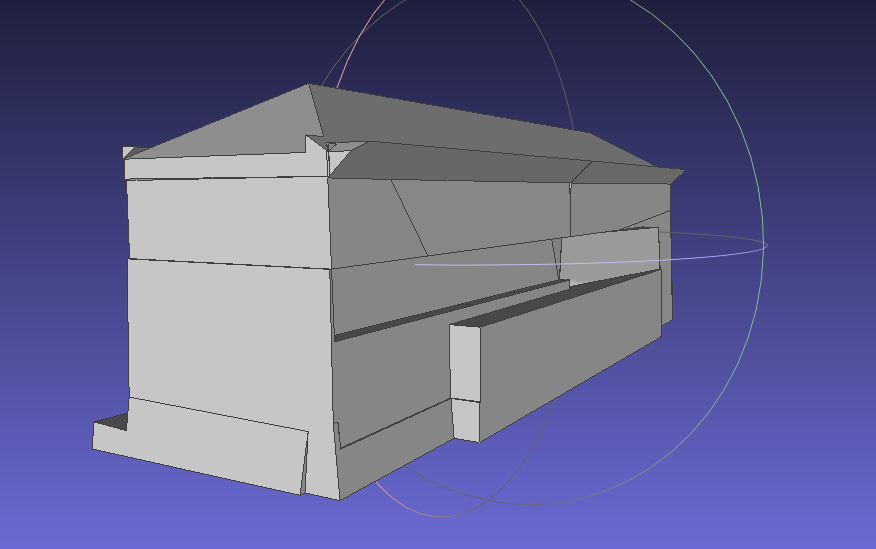
\includegraphics[width=0.25\textwidth]{../../images/screen_kinetic/building_cgal.png}
\hspace{0.05\textwidth}
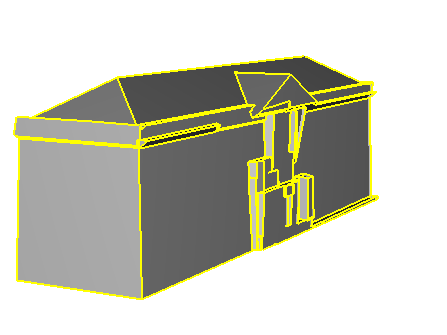
\includegraphics[width=0.25\textwidth]{../../images/screen_kinetic/building_inria.png}
\caption{Visualization of results with a building}
\end{figure}
\begin{figure}[h]
    \centering
    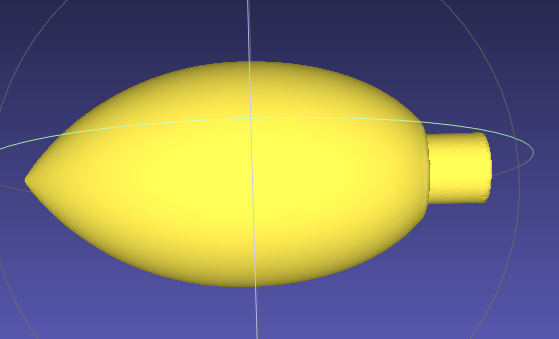
\includegraphics[width=0.25\textwidth]{../../images/screen_kinetic/flame_point.png}
    \hspace{0.05\textwidth}
    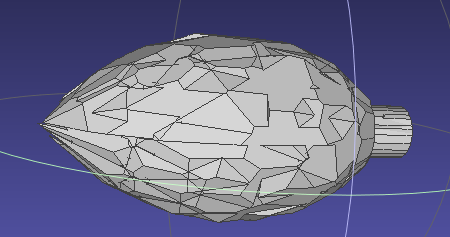
\includegraphics[width=0.29\textwidth]{../../images/screen_kinetic/flame_cgal.png}
    \hspace{0.05\textwidth}
    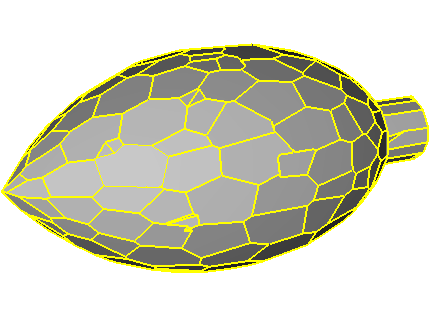
\includegraphics[width=0.22\textwidth]{../../images/screen_kinetic/flame_inria.png}
    \caption{Visualization of results with a flame}
    \end{figure}

\subsection*{Future Perspectives}

    While the results obtained with CGAL and INRIA library data provide valuable insights, it is essential to extend our analysis to data from files in IFC format. We plan to integrate this data into our upcoming experiments to evaluate the performance of the algorithms on real models of buildings and cities.
    
\section{Roadmap}
As of now, we have work to do in order to utilize the Kinetic algorithm in our environment and understand how to apply it correctly. In the following, we will need to work on the following points:
\begin{itemize}
  \item Convert PLT or MSH meshes into a format compatible with the Kinetic algorithm.
  \item If possible, be able to retrieve the labels on the mesh generated by the Kinetic algorithm.
  \item Apply physical theories to the base mesh and the output mesh to analyze the differences between them.
  \item Investigate the feasibility of applying the algorithm on a larger scale, such as a city or a large building, instead of a basic one.
\end{itemize}

    
\nocite{*}
\section{Reference}
\bibliographystyle{plain}
\bibliography{../bibliography/v0/report_bib}
\end{document}